%%%%%%%%%%%%Outline%%%%%%%%%%%%%%%%%%

%%% Section 2.1 The eBPF Execution Pipeline

%%%
% message<eBPF execution pipeline overview>
% Figure 1 shows the eBPF execution pipeline
% user-space compiler turns source code into eBPF bytecode
% kernel verifies bytecode, JIT-compiles to native, attaches to hook point
% program runs each time the kernel invokes the hook

%%% Section 2.2 The eBPF--Native Performance Gap

%%%
% message<runtime cost from ISA-bounded backend and per-opcode JIT>
% pipeline preserves safety but emits slower native code than direct LLVM compilation
% LLVM eBPF backend cannot emit hardware operations the eBPF ISA does not define
% kernel JIT cannot recover them; each opcode translated independently with encoding-level only
% missing-opcode operations decomposed by backend into multiple eBPF instructions
% JIT translates the decomposed instructions one by one to native
% resulting native sequence longer and slower than direct LLVM x86-64/ARM64 backend

%%%%%%%%%%%%Outline%%%%%%%%%%%%%%%%%%

% zhengjie: move 2.2 to section 3

\section{Characterizing the eBPF-Native Performance Gap}
\label{sec:characterization}

Before changing the eBPF execution pipeline, we first characterize the gap
between eBPF bytecode and the hardware operations available to native code.
This section uses pure-bytecode microbenchmarks so that the measurement focuses
on instruction execution rather than application startup or runtime services.
The result is a controlled baseline for the design of \lang: the kernel
execution path has recoverable native-code headroom, but a useful extension
mechanism must expose hardware-friendly operations without bypassing the
verifier.

\subsection{Methodology}
\label{subsec:char-methodology}

We use 29 pure-bytecode microbenchmarks covering compute, branch, local-call,
parser, checksum, string, and packet patterns. Their runtime isolates bytecode
execution and machine-code generation. Each benchmark/runtime pair records
three samples with zero warmups and an inner repeat count of 100000.
Correctness is checked by matching the expected return value and result for
every sample. Runtime ratios use the median steady-state
\texttt{BPF\_PROG\_TEST\_RUN} execution time per benchmark; load, link, and
compile time are excluded from runtime ratios.

The x86-64 and ARM64 pure-bytecode runs compare four execution paths: the
baseline kernel eBPF JIT, a userspace eBPF runtime backed by LLVM-BPF,
userspace native code, and a diagnostic kernel-native execution path.
Table~\ref{tab:char-micro-artifacts} lists the artifacts used for this
characterization.

\begin{table*}[t]
\centering
\scriptsize
\caption{Authoritative pure-bytecode microbenchmark artifacts used for the eBPF-hardware gap characterization. Artifact suffixes identify the result directories under \texttt{micro/results}. Correctness mismatches count expected-result or retval mismatches across all recorded samples.}
\label{tab:char-micro-artifacts}
\begin{tabular}{@{}llllr@{}}
\toprule
Platform & Suite & Artifact suffix & Runtimes & Mismatches \\
\midrule
x86-64 KVM & Pure bytecode 29 & \texttt{210952\_650695} & kernel, LLVM-BPF, native, kernel native & 0 \\
ARM64 AWS & Pure bytecode 29 & \texttt{063319\_954947} & kernel, LLVM-BPF, native, kernel native & 0 \\
\bottomrule
\end{tabular}
\end{table*}


\subsection{RQ1: How Large Is the Pure-Bytecode Headroom?}
\label{subsec:char-pure-bytecode}

\noindent\textbf{Takeaway: pure-bytecode eBPF leaves substantial recoverable
headroom relative to both userspace and kernel-native execution paths.}
On x86-64, userspace native code is 1.716$\times$ faster than the kernel eBPF
JIT, userspace LLVM-BPF is 1.538$\times$ faster, and kernel native is
1.474$\times$ faster (Table~\ref{tab:char-micro-summary}). Figure~\ref{fig:char-pure-aggregate}
shows the same comparison as an aggregate speedup plot. The result is not simply
that running in userspace is faster: the kernel-native path also improves the
same bytecode workloads while staying inside the kernel execution model. We use
this kernel-native path as a diagnostic point, not as the proposed mechanism.

\begin{table*}[t]
\centering
\small
\caption{Pure-bytecode runtime ratios relative to the kernel eBPF JIT. Ratios use median steady-state execution time per benchmark and suite-level geomeans across benchmarks; lower ratio and higher speedup are better.}
\label{tab:char-micro-summary}
\begin{tabular}{@{}lllccc@{}}
\toprule
Platform & Suite & Runtime & Runtime/kernel & Speedup & Wins/losses/ties \\
\midrule
x86-64 KVM & Pure bytecode 29 & Userspace native & 0.583 & 1.716$\times$ & 27/1/1 \\
x86-64 KVM & Pure bytecode 29 & LLVM-BPF userspace & 0.650 & 1.538$\times$ & 27/1/1 \\
x86-64 KVM & Pure bytecode 29 & Kernel native & 0.678 & 1.474$\times$ & 24/2/3 \\
ARM64 AWS & Pure bytecode 29 & Userspace native & 0.467 & 2.141$\times$ & 29/0/0 \\
ARM64 AWS & Pure bytecode 29 & LLVM-BPF userspace & 0.512 & 1.952$\times$ & 29/0/0 \\
ARM64 AWS & Pure bytecode 29 & Kernel native & 0.563 & 1.777$\times$ & 27/0/2 \\
\bottomrule
\end{tabular}
\end{table*}

\begin{figure}[t]
\centering
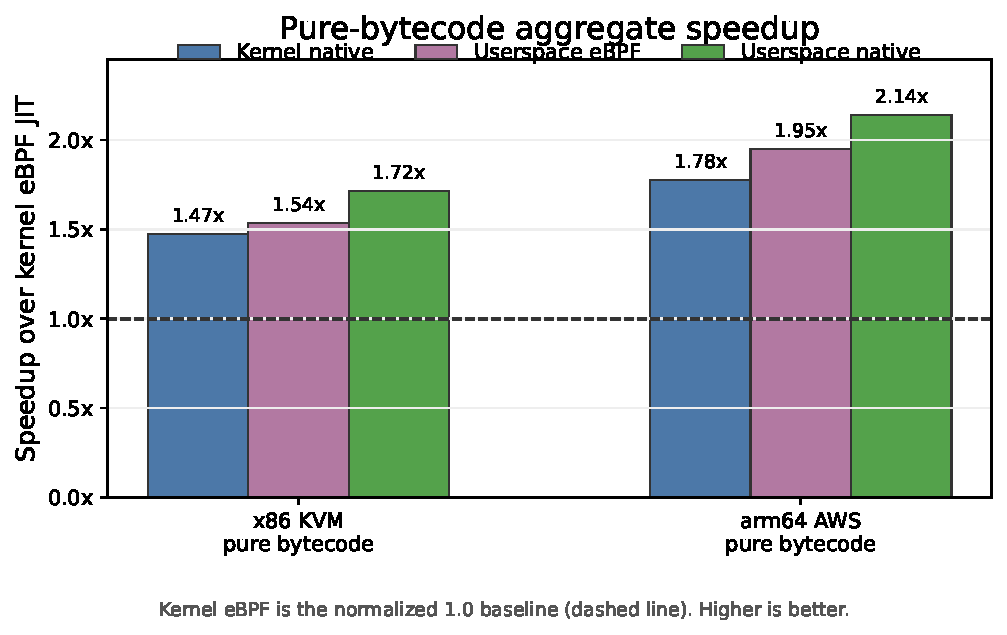
\includegraphics[width=\columnwidth]{figures/sec-3-pure-bytecode-aggregate-20260606.pdf}
\caption{Aggregate pure-bytecode microbenchmark speedup over kernel eBPF JIT. x86 KVM and ARM64 AWS both include kernel native, userspace eBPF, and userspace native. Higher is better; the dashed line is parity.}
\label{fig:char-pure-aggregate}
\end{figure}


\subsection{RQ2: Is the Gap Broad Across Benchmarks?}
\label{subsec:char-percase}

\noindent\textbf{Takeaway: the gap is broad across the suite rather than
driven by one outlier benchmark.}
Most pure-bytecode programs improve under all three non-baseline runtimes:
kernel native wins 24 of 29 x86-64 cases, userspace native wins 27 of 29, and
LLVM-BPF wins 27 of 29 using a $\pm$2\% tie band. Figure~\ref{fig:char-pure-percase}
shows the per-case distribution on x86-64 and ARM64. Machine-code footprint
follows the same direction: kernel native code is 0.541$\times$ the size of
kernel eBPF JIT output on x86-64 pure bytecode and 0.495$\times$ on ARM64 pure
bytecode, confirming that the bytecode execution path emits more machine code
than necessary for many pure instruction workloads.

\begin{figure*}[t]
\centering
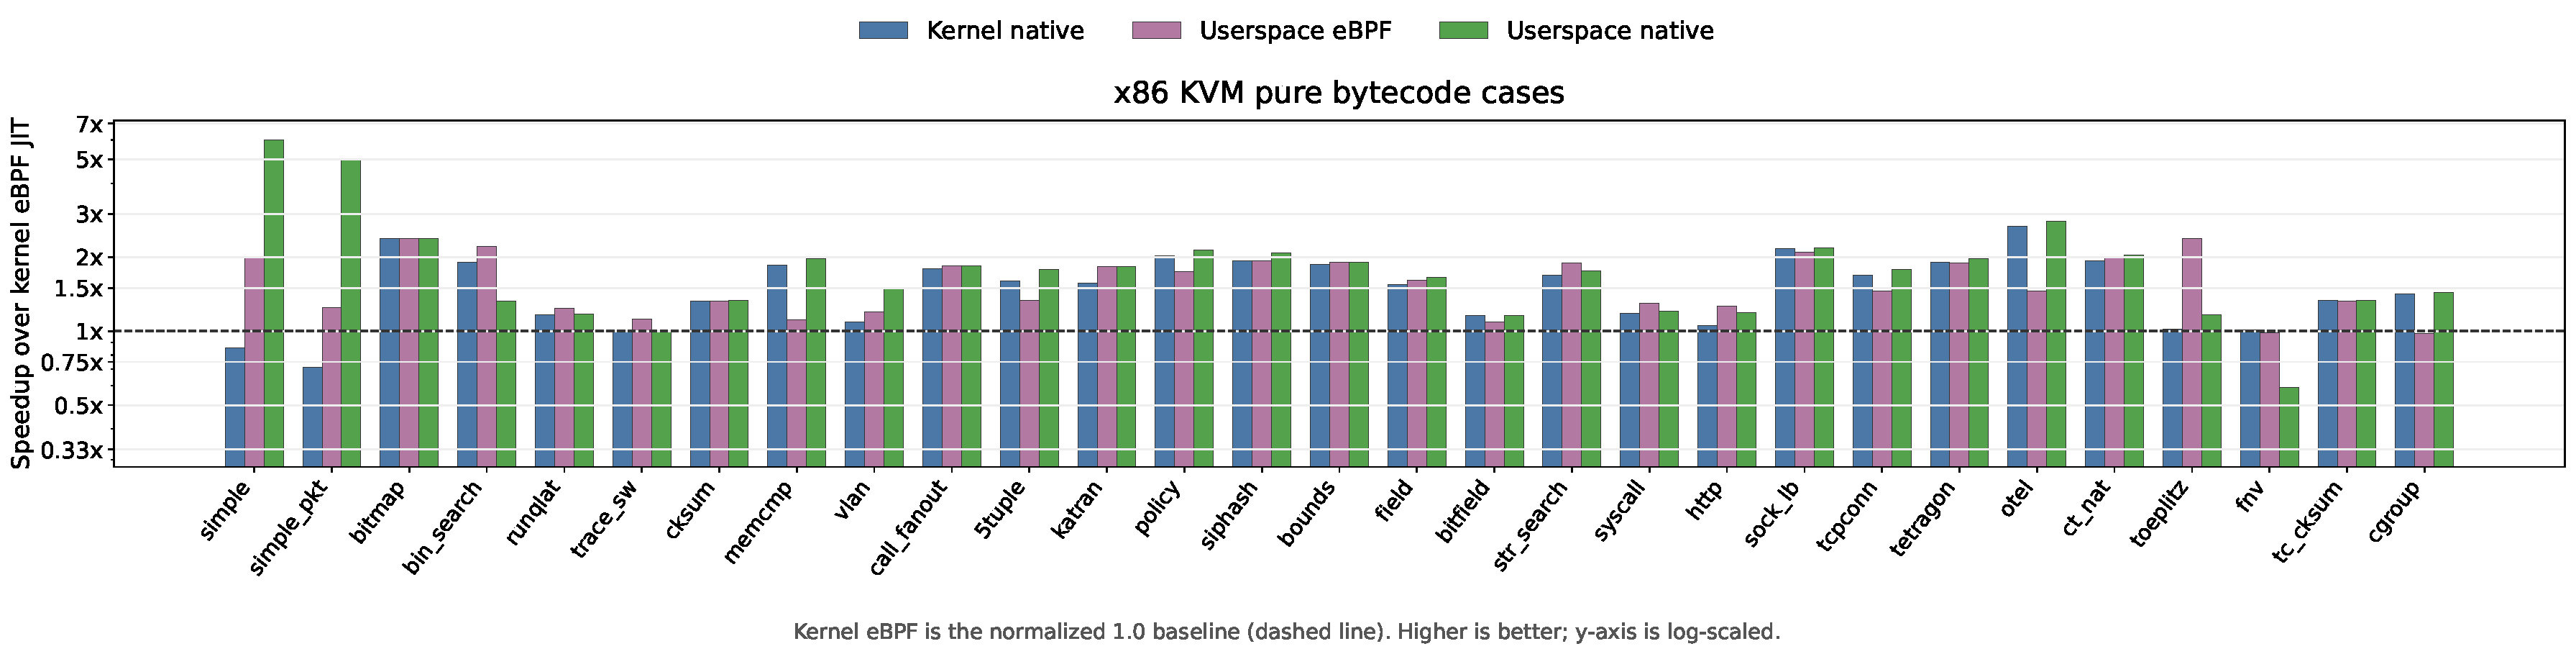
\includegraphics[width=\textwidth]{figures/sec-3-x86-pure-bytecode-percase-20260606.pdf}
\vspace{0.5em}
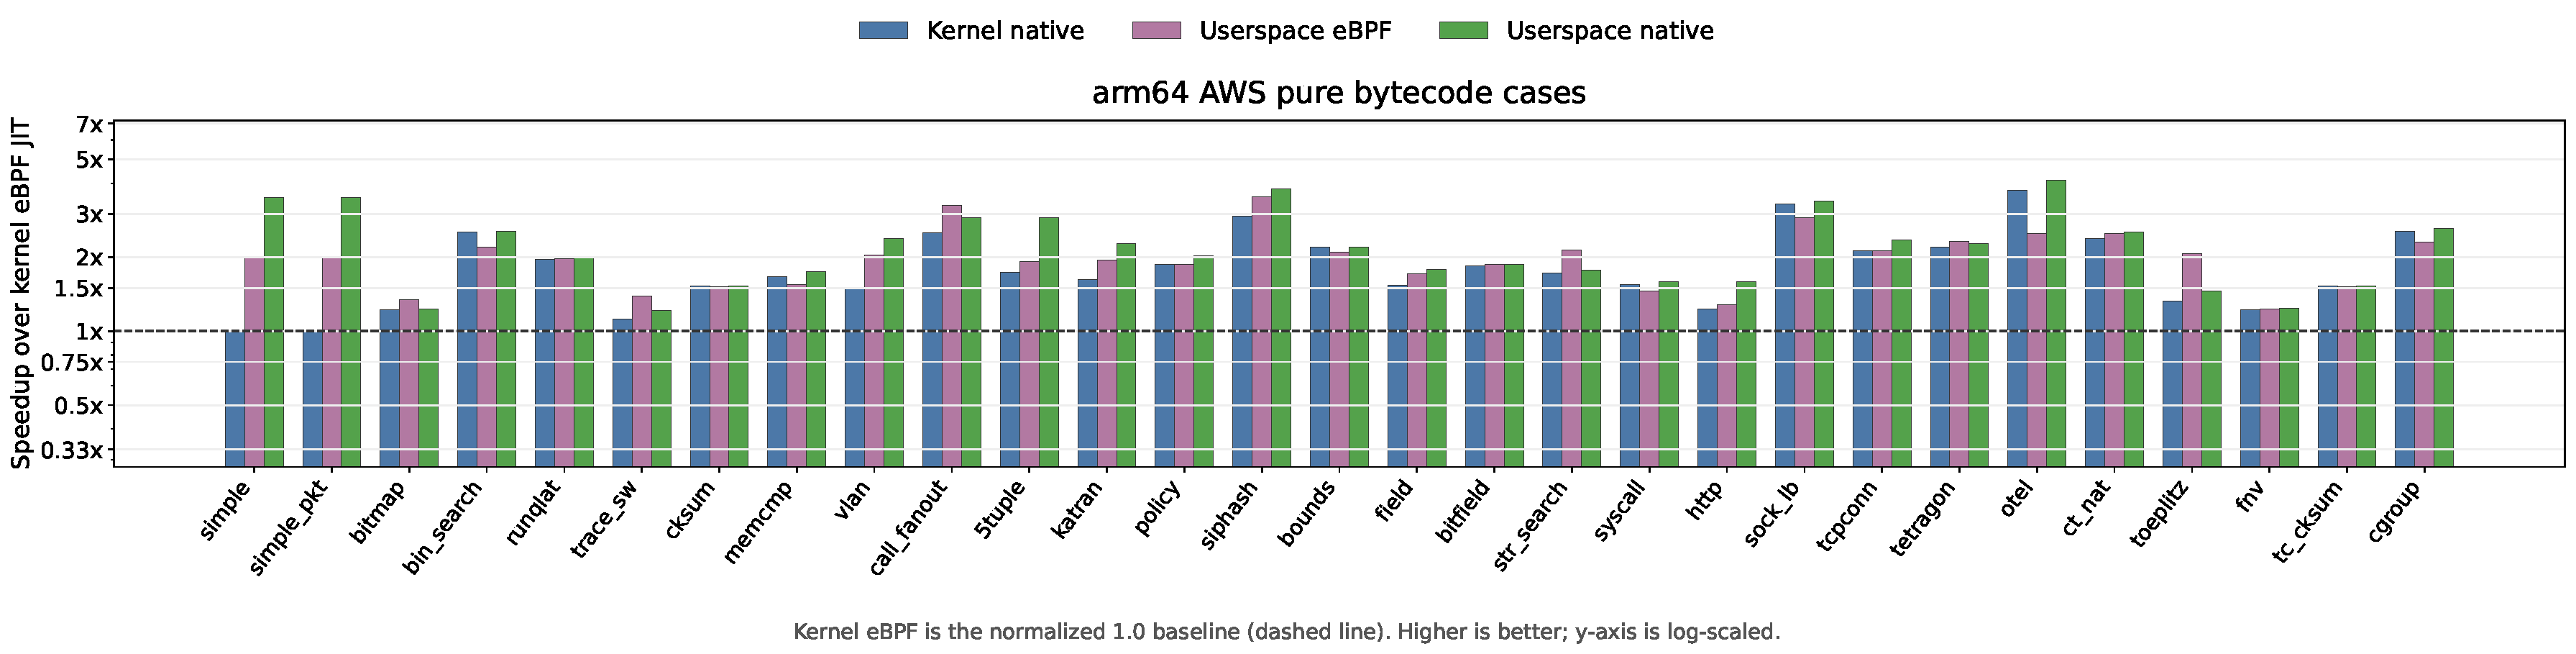
\includegraphics[width=\textwidth]{figures/sec-3-arm64-pure-bytecode-percase-20260606.pdf}
\caption{Per-case pure-bytecode microbenchmark speedup over kernel eBPF JIT. Top: x86 KVM. Bottom: ARM64 AWS. Both platforms report userspace eBPF, userspace native, and kernel native. Higher is better; the dashed line is parity.}
\label{fig:char-pure-percase}
\end{figure*}


\subsection{RQ3: Is the Gap Architecture-Specific?}
\label{subsec:char-portability}

\noindent\textbf{Takeaway: the pure-bytecode headroom is not x86-only.}
ARM64 shows the same qualitative result: userspace native is 2.141$\times$
faster than the ARM64 kernel eBPF JIT, userspace LLVM-BPF is 1.952$\times$
faster, and kernel native is 1.777$\times$ faster with 27 wins and 2 ties
(Table~\ref{tab:char-micro-summary}). This matters for \lang because the
mechanism should expose operation semantics without hard-coding one
architecture's instruction selection into the verifier.

\subsection{RQ4 Case Study: The Missing Rotate Opcode}
\label{subsec:char-rotate}

\noindent\textbf{Takeaway: a missing eBPF opcode forces the compiler to spell
one native hardware operation as a longer bytecode sequence.}
To understand where the slowdown comes from, we examine a concrete example: a
64-bit rotate-left operation, compiled through both pipelines
(Figure~\ref{fig:jit-dump}). The LLVM x86-64 backend recognizes the rotate
idiom and emits a single \texttt{ROL} instruction. The LLVM eBPF backend,
targeting the same source, cannot emit a rotate because the eBPF ISA has no
such opcode. The backend decomposes the operation into eight eBPF instructions,
and the eBPF JIT compiler then translates those instructions one by one to
native code. The two pipelines share the source code, LLVM compiler, and target
hardware; the bottleneck is the missing rotate opcode in the eBPF ISA, not a
local encoding choice in the JIT. Rotate is one instance of a larger ISA
expressiveness gap: Table~\ref{tab:isa-gap} lists five classes of hardware
instructions that have no eBPF opcode equivalent. In each case, the eBPF JIT
compiler must emit a multi-instruction sequence for an operation that the
hardware performs in one or two instructions. This is the gap that \lang
targets: the execution path needs hardware-friendly operations, but the
verifier should still reason over a vanilla eBPF proof sequence.

\begin{figure}[t]
  \centering
  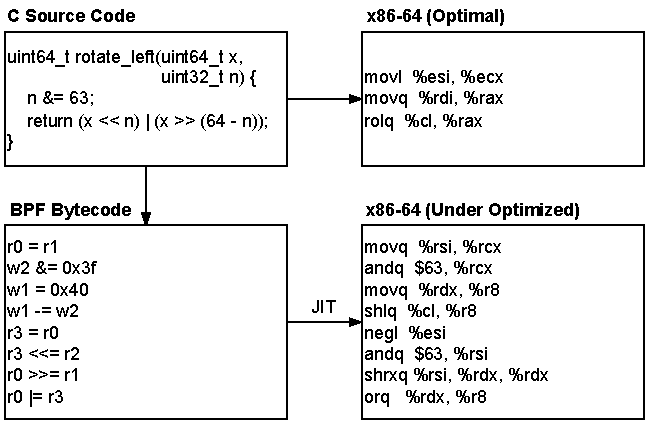
\includegraphics[width=\linewidth]{figures/sec-3-jit-dump.pdf}
  \caption{Compiling a 64-bit rotate through two paths. The direct path compiles C to x86-64 with LLVM, emitting a single \texttt{ROL}. The eBPF path compiles C to eBPF bytecode and then to x86-64 via the eBPF JIT compiler, emitting a longer sequence because the eBPF ISA has no rotate opcode.}
  \label{fig:jit-dump}
\end{figure}

\begin{table}[t]
\centering
\small
\caption{Five classes of hardware instructions with no eBPF opcode. Each row gives the number of eBPF instructions needed to emulate the operation and the corresponding native instructions on x86-64 and ARM64.}
\label{tab:isa-gap}
\begin{tabular}{@{}lccc@{}}
\toprule
Capability & \# eBPF insns & x86-64 & ARM64 \\
\midrule
Conditional move & 3 & \texttt{CMOV} & \texttt{CSEL} \\
Rotate & 8 & \texttt{ROL} & \texttt{ROR} \\
Bitfield extract & 8 & \texttt{SHR+AND} & \texttt{UBFX} \\
Endian load & 10 & \texttt{MOVBE} & \texttt{REV+LDR} \\
Wide recompose & 22 & \texttt{MOV} & \texttt{LDR} \\
\bottomrule
\end{tabular}
\end{table}

\subsection{RQ5: What Should an Extension Preserve?}
\label{subsec:char-implications}

\noindent\textbf{Takeaway: the improvement should come from exposing
hardware-friendly operations without replacing the verifier or changing the
program's kernel execution model.}
The characterization points to a specific design target: the kernel eBPF JIT
has recoverable execution headroom, but that headroom comes from operations the
current ISA cannot express directly. \lang therefore extends the execution
representation with hardware-specific operations while keeping verification
tied to a vanilla eBPF proof sequence. The next section describes that design.